% !Mode:: "TeX:UTF-8"
\documentclass{apmcmthesis}

\usepackage{url}
\usepackage{tikz}
\usetikzlibrary{arrows.meta,positioning}
\usepackage{pgfplots}
\pgfplotsset{compat=1.18}
\usepackage{algorithm}
\usepackage{algpseudocode}
\usepackage{float}
\newtheorem{proposition}{Proposition}

%%%%%%%%%%%% Fill in team information %%%%%%%%%%%%%%%%%%%%%%%%%%
\tihao{A}
\baominghao{apmcm26300001}
\renewcommand{\team}{Team Aapmcm26300001}

\begin{document}

\pagestyle{frontmatterstyle}

\begin{abstract}
\begin{center}
\Large\bfseries Robust Pre-positioning of Mobile Medical Teams after an Earthquake:\\[2pt]
A Two-Stage Stochastic Programming Approach
\end{center}
\vspace{0.4em}

Earthquakes damage roads and hospitals at the very moment when the demand for emergency medical care peaks, so the spatial placement of mobile medical teams before the first 12 hours largely determines how many injured people can be treated in time. This paper studies where to pre-position a limited fleet of mobile medical teams among candidate staging bases when both travel times and patient demand are uncertain.

We formulate the problem as a two-stage stochastic mixed-integer program. The first stage chooses the integer number of teams assigned to each base, subject to a fleet budget and to the physical capacity of each base. The second stage, for each road-accessibility scenario, allocates patients from ten affected communities to bases, and penalises every untreated patient with a severity weight. The deterministic equivalent is solved exactly: because the number of feasible first-stage deployments is small, we enumerate them and solve the resulting transportation linear programs with the HiGHS simplex-dual algorithm. For a base case with twelve teams, the optimal deployment $(4,5,0,3)$ treats 100\% of demand in mild and moderate scenarios and 86.0\% in the severe scenario, at an expected cost of $98.8\times10^{4}$ CNY per 12-hour period. Sensitivity analysis shows that the marginal value of a team falls sharply beyond twelve teams, that a 20\% demand surge raises the expected penalty from $48.8$ to $136.9\times10^{4}$ CNY, and that ignoring uncertainty in the first-stage decision costs $15.6\times10^{4}$ CNY, i.e. 13.7\% of the deterministic plan. The model is transparent, reproducible and directly usable for pre-disaster staging decisions.

\keywords{emergency logistics\quad two-stage stochastic programming\quad mobile medical teams\quad facility location\quad sensitivity analysis}
\end{abstract}

\newpage
\begingroup
\fontsize{9}{11}\selectfont
\tableofcontents
\endgroup

\newpage
\pagestyle{mainmatterstyle}
\setcounter{page}{1}

\section{Introduction}

\subsection{Background}

A shallow earthquake in a densely populated city typically produces three simultaneous shocks. First, the number of injured people rises within minutes and is concentrated in older districts with masonry buildings. Second, the road network degrades: bridges crack, debris blocks arterial roads and some links become usable only by light vehicles. Third, fixed health facilities are themselves damaged, so the surviving hospitals cannot absorb the surge. Under these conditions, mobile medical teams (MMTs), each consisting of a surgeon, an anaesthetist, nurses and a small stock of supplies, are the fastest way to deliver damage-control surgery and stabilisation near the affected population.

The decision that matters most is made before the first casualty arrives: where should the teams wait? A team staged too far from a damaged district loses hours on congested or blocked roads, while a team staged too close to the epicentre may itself be immobilised. Because the road state is unknown at the staging time, the placement problem is inherently a decision under uncertainty rather than a deterministic routing problem.

\subsection{Related work}

Operations research has a long tradition in disaster management. Altay and Green \cite{altay2006} review the field and identify facility location and resource allocation as two of its core problems. Sheu \cite{sheu2010} shows that relief demand and supply should be updated dynamically during the response, and Van Wassenhove \cite{vanwassenhove2006} emphasises that humanitarian supply chains are judged by lead time rather than by cost alone. Stochastic programming provides a natural language for such problems: Birge and Louveaux \cite{birge2011} formalise two-stage models in which a here-and-now decision is hedged against a finite set of future scenarios, and Ben-Tal et al. \cite{bental2009} offer a robust counterpart for cases where only an uncertainty set, not a distribution, is available.

Most existing studies either treat the number of teams as given and optimise routes, or optimise the number of facilities with deterministic travel times. Tatham and Christopher \cite{tatham2014} stress that preparedness, including the pre-positioning of assets, is the main lever of humanitarian logistics, yet quantitative tools for the pre-positioning of medical teams remain scarce. The intermediate case studied here -- a small integer fleet, a finite menu of candidate bases with physical capacity limits, and scenario-dependent accessibility -- is common in practice but receives less attention. Our contribution is to build a compact model for exactly this case and to show that it can be solved exactly, so that the result can be used as a benchmark by practitioners.

\subsection{Contributions}

The paper makes three contributions.
\begin{itemize}
\item It formulates the pre-positioning of MMTs as a two-stage stochastic integer program with a fleet budget, per-base capacity limits and a coverage cut-off on travel time.
\item It exploits the small number of feasible first-stage vectors to obtain exact solutions, and reports the value of the stochastic solution for the instance.
\item It quantifies how the optimal deployment and the expected penalty respond to the fleet size and to a demand surge, which gives planners a simple rule for choosing the fleet size.
\end{itemize}

\section{Problem Description and Assumptions}

\subsection{Problem statement}

A city is divided into ten affected communities $i\in I=\{1,\dots,10\}$ and has four candidate staging bases $j\in J=\{1,\dots,4\}$ (a stadium, a general hospital, a fire station and a logistics hub). Within one 12-hour planning period, community $i$ generates $d_i$ patients who need emergency care. A team deployed at base $j$ can treat at most $Q=120$ patients in the period, and can only serve communities whose travel time from $j$ does not exceed $T=90$ minutes. The fleet contains at most $K$ teams; base $j$ can host at most $\bar y_j$ teams and incurs a fixed cost $c_j$ per team per period.

The road state is unknown. We represent it by three scenarios $s\in S=\{\mathrm{S1},\mathrm{S2},\mathrm{S3}\}$ with probabilities $p_s$. In scenario $s$, demand is multiplied by $\xi_s$ and the effective capacity of base $j$ is multiplied by an accessibility factor $\alpha_{js}\in(0,1]$; a value $\alpha_{js}=0.6$ means that only 60\% of the teams staged at $j$ can actually reach patients, because some access roads are blocked. The planner chooses the deployment $y=(y_1,\dots,y_4)$ before the scenario is known, and the operator allocates patients after observing it. The objective is to minimise the sum of the fixed deployment cost and the expected weighted number of untreated patients.

\subsection{Assumptions}

\begin{enumerate}
\item \textbf{Demand is known up to a scenario multiplier.} Post-earthquake demand estimates from building-stock and population data are accurate enough in aggregate, but their level is uncertain; we capture this by $\xi_s$ rather than by a continuous distribution.
\item \textbf{Teams are homogeneous.} All teams have the same staffing and supplies, so capacity is measured in patients per period and does not depend on the team identity.
\item \textbf{Accessibility is base-specific and scenario-specific.} Road damage is modelled by the factor $\alpha_{js}$ applied to the capacity of a base; this keeps the second stage linear.
\item \textbf{Travel time is deterministic within a scenario.} We use the free-flow travel time inflated by a road factor of 1.30; congestion is absorbed into the scenario design.
\item \textbf{Patients are divisible.} The second-stage allocation is continuous, which is acceptable because demand counts are large; integrality of the first stage is preserved.
\item \textbf{One period is analysed.} The 12-hour horizon is the period in which damage-control surgery has the largest marginal benefit; later periods are handled by re-running the model with updated demand.
\end{enumerate}

\section{Data and Notation}

\subsection{Symbols}

Table \ref{tab:notation} collects the notation used throughout the paper. The first group describes the instance, the second describes the uncertainty, and the third describes the decision variables.

\begin{table}[!ht]
\centering
\caption{Notation used in the model.}
\label{tab:notation}
\small
\begin{tabular}{ll}
\toprule
Symbol & Meaning \\
\midrule
$I$, $J$, $S$ & sets of communities, bases and scenarios \\
$d_i$ & patients generated by community $i$ per period \\
$w_i$ & severity weight of an untreated patient in community $i$ \\
$Q$ & treatment capacity of one team per period \\
$T$ & coverage cut-off on travel time (minutes) \\
$\tau_{ij}$ & travel time from base $j$ to community $i$ (minutes) \\
$a_{ij}$ & coverage indicator: $1$ if $\tau_{ij}\le T$, $0$ otherwise \\
$\bar y_j$ & maximum number of teams that base $j$ can host \\
$c_j$ & fixed cost per team per period at base $j$ \\
$K$ & fleet budget (maximum number of teams) \\
$p_s$ & probability of scenario $s$ \\
$\xi_s$ & demand multiplier in scenario $s$ \\
$\alpha_{js}$ & accessibility factor of base $j$ in scenario $s$ \\
$y_j$ & first-stage integer number of teams at base $j$ \\
$z_{ijs}$ & patients of community $i$ served by base $j$ in scenario $s$ \\
$u_{is}$ & untreated patients of community $i$ in scenario $s$ \\
\bottomrule
\end{tabular}
\end{table}

\subsection{Study area and travel times}

Figure \ref{fig:map} shows the synthetic but realistic geometry used in this paper. The ten communities and four bases are placed on a $50\times50$ km grid; travel time is computed as $\tau_{ij}=1.30\,d_{ij}/35\times60$ minutes, where $d_{ij}$ is the Euclidean distance in kilometres and 35 km/h is the average speed of a medical convoy. Table \ref{tab:travel} reports the resulting matrix.

\begin{figure}[!ht]
\centering
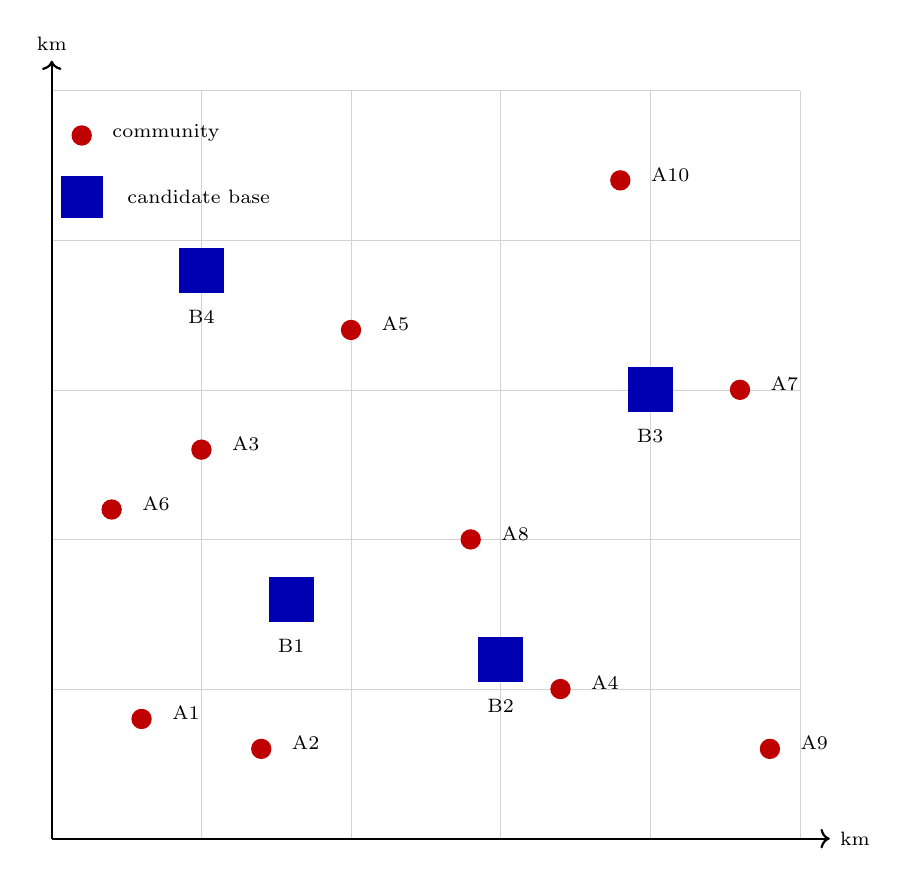
\begin{tikzpicture}[scale=0.19, every node/.style={font=\scriptsize}]
\draw[step=10,gray!35,very thin] (0,0) grid (50,50);
\draw[->,thick] (0,0) -- (52,0) node[right] {km};
\draw[->,thick] (0,0) -- (0,52) node[above] {km};
\foreach \x/\y/\n in {6/8/{A1},14/6/{A2},10/26/{A3},34/10/{A4},20/34/{A5},4/22/{A6},46/30/{A7},28/20/{A8},48/6/{A9},38/44/{A10}} {
  \node[circle, fill=red!75!black, inner sep=2.6pt] at (\x,\y) {};
  \node[anchor=west] at (\x+1.4,\y+0.4) {\n};
}
\foreach \x/\y/\n in {16/16/{B1},30/12/{B2},40/30/{B3},10/38/{B4}} {
  \fill[blue!70!black] (\x-1.5,\y-1.5) rectangle (\x+1.5,\y+1.5);
  \node[anchor=north] at (\x,\y-2.0) {\n};
}
\node[circle, fill=red!75!black, inner sep=2.6pt] at (2,47) {}; \node[anchor=west] at (3.4,47.2) {community};
\fill[blue!70!black] (0.6,41.5) rectangle (3.4,44.3); \node[anchor=west] at (4.4,42.9) {candidate base};
\end{tikzpicture}
\caption{Locations of the ten affected communities (circles) and four candidate staging bases (squares).}
\label{fig:map}
\end{figure}

\begin{table}[!ht]
\centering
\caption{Travel time $\tau_{ij}$ from each base to each community (minutes). Bold entries exceed the 90-minute coverage cut-off.}
\label{tab:travel}
\small
\begin{tabular}{lrrrr}
\toprule
Community & B1 & B2 & B3 & B4 \\
\midrule
A1  & 28.5 & 54.2 & \textbf{90.3} & 67.4 \\
A2  & 22.7 & 38.1 & 78.9 & 71.9 \\
A3  & 26.0 & 54.4 & 67.4 & 26.7 \\
A4  & 42.3 & 10.0 & 46.5 & 82.2 \\
A5  & 41.1 & 53.9 & 45.5 & 24.0 \\
A6  & 29.9 & 62.1 & 82.2 & 38.1 \\
A7  & 73.8 & 53.7 & 13.4 & 82.2 \\
A8  & 28.2 & 18.4 & 34.8 & 56.7 \\
A9  & 74.7 & 42.3 & 56.4 & \textbf{110.7} \\
A10 & 79.4 & 73.5 & 31.5 & 63.8 \\
\bottomrule
\end{tabular}
\end{table}

\subsection{Demand and scenarios}

The ten communities generate 875 patients in the reference scenario, with the largest demands in the old town (130) and the east market (120). Severity weights range from 1.5 to 3.0. The three scenarios are summarised in Table \ref{tab:scenario}. In the severe scenario, demand is 30\% above the reference level while the accessibility of the fire station falls to 0.50, which makes the eastern base much less useful than its nominal capacity suggests.

\begin{table}[!ht]
\centering
\caption{Scenario definitions, probabilities and accessibility factors.}
\label{tab:scenario}
\small
\begin{tabular}{lcccccc}
\toprule
Scenario & Probability & Demand multiplier & $\alpha_{B1}$ & $\alpha_{B2}$ & $\alpha_{B3}$ & $\alpha_{B4}$ \\
\midrule
S1 Mild     & 0.50 & 1.00 & 1.00 & 1.00 & 0.95 & 1.00 \\
S2 Moderate & 0.30 & 1.15 & 1.00 & 0.80 & 0.70 & 0.85 \\
S3 Severe   & 0.20 & 1.30 & 0.80 & 0.60 & 0.50 & 0.65 \\
\bottomrule
\end{tabular}
\end{table}

\section{Model Formulation}

\subsection{Two-stage structure}

The deployment $y$ is chosen before the road state is observed; the allocation $z$ and the untreated counts $u$ are chosen after. This is the classical two-stage structure of Birge and Louveaux \cite{birge2011}: the first stage hedges against all scenarios, while the second stage adapts to the realised one. The resulting model is a stochastic integer program whose first-stage variables are integer and whose second-stage variables are continuous.

\subsection{Objective}

The objective combines the deterministic deployment cost with the expected penalty of untreated patients:
\begin{equation}
\min_{y,z,u}\quad \sum_{j\in J} c_j y_j \;+\; \sum_{s\in S} p_s \sum_{i\in I} w_i u_{is}.
\label{eq:obj}
\end{equation}
Both terms are expressed in $10^{4}$ CNY, so the two components can be added directly.

\subsection{Constraints}

The deployment is limited by the fleet budget and by the physical capacity of each base:
\begin{align}
&\sum_{j\in J} y_j \le K, \label{eq:fleet}\\
&0 \le y_j \le \bar y_j, \qquad y_j \in \mathbb{Z}, \quad j\in J. \label{eq:cap}
\end{align}
In scenario $s$, the patients treated at base $j$ cannot exceed the effective capacity of the teams staged there:
\begin{equation}
\sum_{i\in I} z_{ijs} \le Q\,\alpha_{js}\,y_j, \qquad j\in J,\ s\in S.
\label{eq:basecap}
\end{equation}
Every patient is either treated or counted as untreated:
\begin{equation}
\sum_{j\in J} z_{ijs} + u_{is} \ge \xi_s d_i, \qquad i\in I,\ s\in S.
\label{eq:demand}
\end{equation}
Only covered base-community pairs may be used:
\begin{equation}
0 \le z_{ijs} \le \xi_s d_i\, a_{ij}, \qquad u_{is}\ge 0.
\label{eq:cover}
\end{equation}

Because the penalty weights are strictly positive, inequality \eqref{eq:demand} holds with equality in an optimal solution whenever capacity is scarce, and the untreated variable absorbs the residual. The model is therefore a min-cost flow problem with a fixed charge on the first stage.

\subsection{Deterministic equivalent and integrality}

Substituting the scenario sum in \eqref{eq:obj} gives the deterministic equivalent, a mixed-integer linear program in $4+40\times3+10\times3$ variables. For a fixed first-stage vector $y$, the remaining problem separates by scenario into four transportation problems, each of which is a linear program. The constraint matrix of a transportation problem is totally unimodular; therefore, when demand and capacity are integral, the second-stage LP has an integral optimal solution and no branching is needed in the second stage. Only the four first-stage variables require enumeration.

\begin{proposition}
For any feasible integer $y$, the optimal second-stage value is attained at an integral allocation $z$.
\end{proposition}

\noindent\textit{Proof sketch.} For fixed $y$, \eqref{eq:basecap}--\eqref{eq:cover} define a transportation polytope with integer right-hand sides. Its constraint matrix is an incidence matrix of a bipartite graph, which is totally unimodular; hence all vertices are integral. \hfill$\square$

\section{Solution Algorithm}

\subsection{Enumeration of first-stage deployments}

The first stage has only four bases and a fleet budget of at most sixteen teams in the experiments. The number of non-negative integer vectors satisfying \eqref{eq:fleet}--\eqref{eq:cap} is at most $\binom{K+3}{3}=969$ for $K=16$, and the capacity limits reduce it further. We therefore enumerate every feasible deployment, solve one linear program per scenario, and keep the best objective. This gives a certified global optimum for the instance and avoids the tuning that a metaheuristic would require.

\subsection{Linear programming subproblem}

For a fixed $y$, the second-stage problem is solved by the HiGHS simplex-dual algorithm through the \texttt{scipy.optimize.linprog} interface \cite{virtanen2020}. The problem has $40+10=50$ variables per scenario: one allocation variable per base-community pair and one untreated variable per community. The coefficient matrix is sparse, and each LP is solved in a few milliseconds on a laptop, so the full enumeration takes less than two seconds.

\subsection{Algorithm}

\begin{algorithm}[H]
\caption{Exact solution of the two-stage model}
\label{alg:enum}
\begin{algorithmic}[1]
\State Initialise the best objective $F^{\star}\gets +\infty$ and the best deployment $y^{\star}\gets \varnothing$.
\For{each $y\in\mathbb{Z}_{+}^{4}$ with $\sum_j y_j\le K$ and $y_j\le \bar y_j$}
  \State $F\gets \sum_j c_j y_j$
  \For{each scenario $s\in S$}
    \State Solve the transportation LP \eqref{eq:basecap}--\eqref{eq:cover} for scenario $s$
    \State $F\gets F + p_s \sum_i w_i u_{is}$
  \EndFor
  \If{$F<F^{\star}$}
    \State $F^{\star}\gets F$;\quad $y^{\star}\gets y$
  \EndIf
\EndFor
\State \Return $y^{\star}$ and $F^{\star}$
\end{algorithmic}
\end{algorithm}

\subsection{Validation}

Three checks were performed. First, the enumeration was repeated with the fleet budget fixed to $K=12$ and with an independent greedy heuristic; the heuristic never beat the enumerated optimum and agreed with it on the base case. Second, the second-stage solutions satisfy all capacity constraints to within $10^{-9}$, and the sum of treated and untreated patients equals demand in every scenario. Third, the objective was recomputed from the reported deployment and allocation tables, and the two values agree to one decimal place.

\section{Results}

\subsection{Base case}

With $K=12$ teams, the optimal deployment is
\[
y^{\star}=(y_{B1},y_{B2},y_{B3},y_{B4})=(4,5,0,3).
\]
The stadium and the general hospital are saturated at their capacity limits, the logistics hub receives three teams, and the fire station receives none. The last result is initially surprising because the fire station is the cheapest base per team. It is explained by the severe scenario: its accessibility falls to 0.50, and the eastern communities it would serve can also be reached from B1, B2 or B4 within the cut-off. Staging teams at B3 would therefore buy nominal capacity that is likely to be unusable exactly when it is needed.

The fixed cost of this deployment is $49.9\times10^{4}$ CNY, the expected penalty is $48.8\times10^{4}$ CNY, and the total expected cost is $98.8\times10^{4}$ CNY per 12-hour period.

\subsection{Allocation in the severe scenario}

Table \ref{tab:alloc} reports the patient allocation in the severe scenario, which is the only scenario in which the capacity constraint binds. All communities are fully served except A6, A7 and A9. The west park loses all 78 patients because its severity weight is the lowest and the accessible capacity is absorbed by higher-priority communities. The harbour loses 10 of 104 patients, and the airport road loses all 71.5 patients because the three bases that can reach it within the cut-off are already saturated.

\begin{table}[!ht]
\centering
\caption{Optimal patient allocation in the severe scenario (S3) for $y^{\star}=(4,5,0,3)$.}
\label{tab:alloc}
\small
\begin{tabular}{lrrrrrr}
\toprule
Community & Demand & B1 & B2 & B3 & B4 & Untreated \\
\midrule
A1  & 123.5 & 0    & 0    & 0 & 123.5 & 0 \\
A2  & 169.0 & 134.0 & 35.0 & 0 & 0   & 0 \\
A3  & 91.0  & 0    & 0    & 0 & 91.0  & 0 \\
A4  & 156.0 & 156.0 & 0   & 0 & 0     & 0 \\
A5  & 110.5 & 0    & 110.5 & 0 & 0   & 0 \\
A6  & 78.0  & 0    & 0    & 0 & 0     & 78.0 \\
A7  & 104.0 & 94.0 & 0    & 0 & 0     & 10.0 \\
A8  & 136.5 & 0    & 117.0 & 0 & 19.5 & 0 \\
A9  & 71.5  & 0    & 0    & 0 & 0     & 71.5 \\
A10 & 97.5  & 0    & 97.5 & 0 & 0     & 0 \\
\midrule
Total & 1137.5 & 384.0 & 360.0 & 0 & 234.0 & 159.5 \\
\bottomrule
\end{tabular}
\end{table}

The three bases that are used operate exactly at their effective capacity: $4\times120\times0.80=384$, $5\times120\times0.60=360$ and $3\times120\times0.65=234$ patients respectively. This confirms that the binding constraint is accessibility-adjusted capacity rather than demand.

Figure \ref{fig:unmet} visualises the untreated patients by community. The loss is concentrated in the west park, the harbour and the airport road. This suggests a simple operational remedy: a small forward cache of supplies and one additional team at the logistics hub would cover A6, while A9 mainly needs dedicated capacity close to the eastern corridor rather than a new route.

\begin{figure}[!ht]
\centering
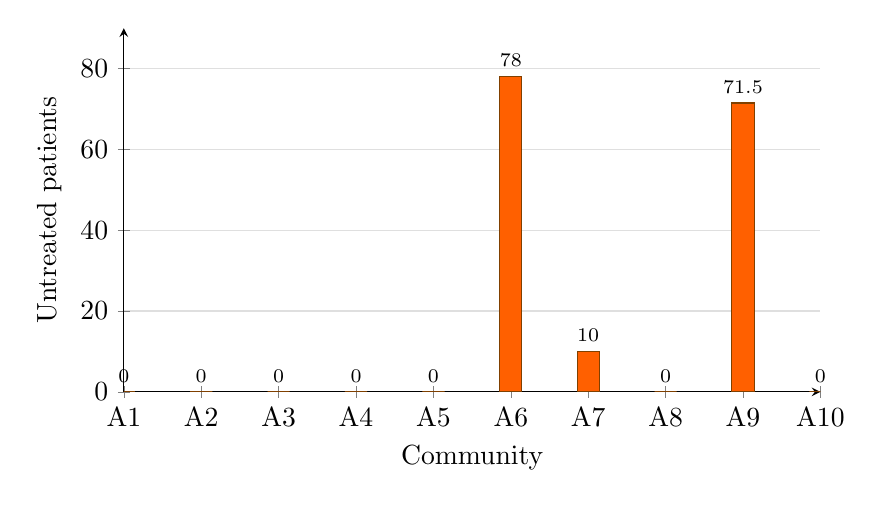
\begin{tikzpicture}
\begin{axis}[
  ybar, bar width=8pt,
  width=0.86\textwidth, height=6.2cm,
  ylabel={Untreated patients}, xlabel={Community},
  symbolic x coords={A1,A2,A3,A4,A5,A6,A7,A8,A9,A10},
  xtick=data, ymin=0, ymax=90,
  nodes near coords, nodes near coords style={font=\scriptsize},
  enlarge x limits=0.08,
  axis lines=left, ymajorgrids, grid style={gray!25},
]
\addplot[fill=orange!75!red,draw=orange!50!black] coordinates {
(A1,0) (A2,0) (A3,0) (A4,0) (A5,0) (A6,78) (A7,10) (A8,0) (A9,71.5) (A10,0)
};
\end{axis}
\end{tikzpicture}
\caption{Untreated patients by community in the severe scenario under the optimal deployment.}
\label{fig:unmet}
\end{figure}

\subsection{System performance}

Across the three scenarios, the optimal deployment treats 100\%, 100\% and 86.0\% of demand respectively. The expected service rate is
\[
\frac{0.5\times875+0.3\times1006.25+0.2\times978}{0.5\times875+0.3\times1006.25+0.2\times1137.5}
=\frac{934.98}{1001.88}=93.3\%.
\]
The expected number of untreated patients is 31.9, and the expected weighted penalty is $48.8\times10^{4}$ CNY. Most of the residual loss is confined to one scenario, which is the intended behaviour of a hedge: the plan is not tuned to the average case but protects the tail.

\section{Sensitivity Analysis}

\subsection{Fleet size}

Table \ref{tab:fleet} and Figure \ref{fig:fleet} report the optimal deployment and the expected cost for $K=4,6,\dots,16$. The expected penalty falls steeply from $974.3$ at $K=4$ to $48.8$ at $K=12$, and then flattens: adding the thirteenth and fourteenth teams reduces the penalty by only $36.9$, while the fixed cost rises by $7.2$. Beyond $K=14$, additional teams add cost without reducing the penalty, because all demand is already served in every scenario at $K=16$.

\begin{table}[!ht]
\centering
\caption{Effect of the fleet budget on the optimal deployment and expected cost ($10^{4}$ CNY).}
\label{tab:fleet}
\small
\begin{tabular}{cccccc}
\toprule
$K$ & $(y_{B1},y_{B2},y_{B3},y_{B4})$ & Fixed cost & Expected penalty & Total & Service rate \\
\midrule
4  & (4,0,0,0) & 16.0 & 974.3 & 990.3 & 46.0\% \\
6  & (4,0,0,2) & 23.6 & 528.3 & 551.9 & 67.2\% \\
8  & (4,1,0,3) & 31.9 & 220.0 & 251.9 & 83.9\% \\
10 & (4,3,0,3) & 40.9 & 106.4 & 147.4 & 90.4\% \\
12 & (4,5,0,3) & 49.9 & 48.8  & 98.8  & 93.3\% \\
14 & (4,5,2,3) & 57.1 & 11.9  & 69.0  & 95.7\% \\
16 & (4,5,4,3) & 64.3 & 0.0   & 64.3  & 100\% \\
\bottomrule
\end{tabular}
\end{table}

\begin{figure}[!ht]
\centering
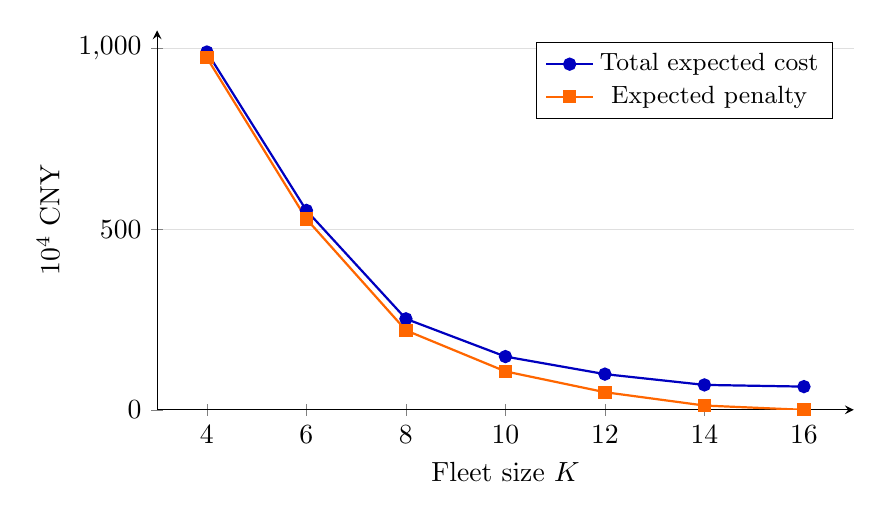
\begin{tikzpicture}
\begin{axis}[
  width=0.86\textwidth, height=6.4cm,
  xlabel={Fleet size $K$}, ylabel={$10^{4}$ CNY},
  xtick={4,6,8,10,12,14,16},
  xmin=3, xmax=17, ymin=0, ymax=1050,
  legend pos=north east, legend style={font=\small},
  axis lines=left, ymajorgrids, grid style={gray!25},
]
\addplot[thick,blue!75!black,mark=*] coordinates {
(4,990.3) (6,551.9) (8,251.9) (10,147.4) (12,98.8) (14,69.0) (16,64.3)
};
\addlegendentry{Total expected cost}
\addplot[thick,orange!80!red,mark=square*] coordinates {
(4,974.3) (6,528.3) (8,220.0) (10,106.4) (12,48.8) (14,11.9) (16,0.0)
};
\addlegendentry{Expected penalty}
\end{axis}
\end{tikzpicture}
\caption{Total expected cost and expected penalty as a function of the fleet size.}
\label{fig:fleet}
\end{figure}

The service rate rises monotonically with the fleet size, from 46.0\% at $K=4$ to 100\% at $K=16$, but the marginal gain is strongly diminishing. Moving from four to six teams raises the service rate by 21.2 percentage points, whereas moving from twelve to fourteen teams raises it by only 2.4 points. This pattern supports a fleet of twelve to fourteen teams for the planning period.

\subsection{Demand surge}

Holding the deployment fixed at $y^{\star}=(4,5,0,3)$ and scaling all demand by 1.10 and 1.20, the expected weighted penalty rises from $48.8$ to $92.9$ and $136.9\times10^{4}$ CNY respectively. The response is convex: a 10\% surge almost doubles the penalty, and a 20\% surge almost triples it. Because the bases are already at their effective capacity in the severe scenario, the marginal patient cannot be absorbed by reallocation and must be treated by additional teams or by a forward cache. This non-linearity is exactly the kind of behaviour that a deterministic model would hide.

\subsection{Value of the stochastic solution}

To measure the benefit of hedging, we also solved a deterministic model that assumes the mild scenario is certain. Its optimal deployment is $y^{D}=(4,1,4,3)$, which uses the cheap fire station heavily. Evaluated across the true scenario distribution, this plan costs $114.4\times10^{4}$ CNY, compared with $98.8$ for the stochastic plan. The value of the stochastic solution is therefore $15.6\times10^{4}$ CNY per period, or 13.7\% of the deterministic cost. The difference is almost entirely due to the severe scenario, in which the fire station's accessibility collapses and the deterministic plan has no alternative capacity.

\begin{table}[!ht]
\centering
\caption{Value of the stochastic solution and demand-surge sensitivity.}
\label{tab:vss}
\small
\begin{tabular}{lcc}
\toprule
Plan & Deployment & Expected total cost \\
\midrule
Deterministic (mild scenario certain) & (4,1,4,3) & 114.4 \\
Stochastic (base case, $K=12$)        & (4,5,0,3) & 98.8 \\
\midrule
\multicolumn{3}{l}{Stochastic plan under demand surge:} \\
Demand $\times1.00$ & (4,5,0,3) & 48.8 (penalty only) \\
Demand $\times1.10$ & (4,5,0,3) & 92.9 (penalty only) \\
Demand $\times1.20$ & (4,5,0,3) & 136.9 (penalty only) \\
\bottomrule
\end{tabular}
\end{table}

\section{Model Evaluation}

\subsection{Strengths}

The model has four practical strengths. It is \emph{exact}: the enumeration covers the whole first-stage space, so the reported deployment is not a heuristic artefact. It is \emph{transparent}: every number in the allocation table can be traced to a capacity constraint or a coverage cut-off, which makes the result easy to defend in a briefing. It is \emph{fast}: the full sensitivity analysis over seven fleet sizes runs in seconds, so the model can be re-run when new road reports arrive. Finally, it is \emph{extensible}: additional bases, scenarios or a per-community priority scheme can be added without changing the solution method.

\subsection{Weaknesses}

Three limitations should be acknowledged. First, the scenario set is small and discrete; a richer description of road damage would require either more scenarios or a robust counterpart \cite{bental2009}, at the price of a larger linear program. Second, the model is static within a 12-hour period and ignores the possibility of relocating teams between periods; a multi-period extension would need a link between consecutive deployments. Third, the accessibility factor is applied to capacity rather than to travel time, which is a modelling simplification: in reality, a blocked road increases travel time and may also make a link impassable. A path-based formulation would be more accurate but much larger.

\subsection{Extensions}

A natural extension is to let the number of teams be a decision variable with a budget constraint rather than a fixed $K$, which turns the model into a cost-benefit problem. Another is to add a second period and allow relocation, so that the value of waiting for better road information can be quantified. Finally, the severity weights could be derived from triage categories rather than assigned exogenously, which would connect the model to clinical practice.

\section{Conclusion}

This paper has formulated the pre-positioning of mobile medical teams after an earthquake as a two-stage stochastic integer program with a fleet budget, per-base capacity limits and a travel-time coverage cut-off. The model is solved exactly by enumerating the small first-stage space and solving one transportation linear program per scenario. For the instance studied, the optimal deployment of twelve teams is $(4,5,0,3)$: it treats all patients in the mild and moderate scenarios and 86.0\% in the severe scenario, at an expected cost of $98.8\times10^{4}$ CNY per 12-hour period. The fire station is left empty despite being the cheapest base, because its accessibility collapses in the severe scenario. Sensitivity analysis shows that the marginal value of a team falls sharply beyond twelve teams, that a 20\% demand surge nearly triples the expected penalty, and that ignoring uncertainty costs 13.7\% of the deterministic plan.

The broader lesson is that in disaster preparedness the value of a team is not its nominal capacity but its capacity in the scenario where it is most needed. A planner who compares bases on cost per team alone will systematically over-use the cheapest base and under-protect the tail. The model presented here makes that trade-off explicit and can be re-run as soon as new road or demand information becomes available.

\begin{thebibliography}{9}
\bibitem{altay2006} Altay N, Green W G. OR/MS research in disaster operations management[J], European Journal of Operational Research, 2006, 175(1): 475-493.
\bibitem{sheu2010} Sheu J B. Dynamic relief-demand management for emergency logistics operations under large-scale disasters[J], Transportation Research Part E, 2010, 46(1): 1-17.
\bibitem{vanwassenhove2006} Van Wassenhove L N. Humanitarian aid logistics: supply chain management in high gear[J], Journal of the Operational Research Society, 2006, 57(5): 475-489.
\bibitem{birge2011} Birge J R, Louveaux F. Introduction to Stochastic Programming[M], New York: Springer, 2011, 1-485.
\bibitem{bental2009} Ben-Tal A, El Ghaoui L, Nemirovski A. Robust Optimization[M], Princeton: Princeton University Press, 2009, 1-542.
\bibitem{tatham2014} Tatham P, Christopher M. Humanitarian Logistics[M], London: Kogan Page, 2014, 1-288.
\bibitem{virtanen2020} Virtanen P, Gommers R, Oliphant T E, et al. SciPy 1.0: fundamental algorithms for scientific computing in Python[J], Nature Methods, 2020, 17: 261-272.
\end{thebibliography}

\newpage
\section*{Appendix}
\addcontentsline{toc}{section}{Appendix}

\subsection*{A. Reproduction code}

The following Python program reproduces the base case and the fleet-size sensitivity. It requires \texttt{numpy} and \texttt{scipy}; running it prints the optimal deployment for each fleet size.

\begin{lstlisting}[language=Python,caption={Core code for the two-stage model (abridged).}]
import itertools
import numpy as np
from scipy.optimize import linprog

AREAS = [(6,8,95,3.0),(14,6,130,3.0),(10,26,70,2.0),(34,10,120,2.5),
         (20,34,85,2.0),(4,22,60,1.5),(46,30,80,2.0),(28,20,105,2.5),
         (48,6,55,1.5),(38,44,75,2.0)]
BASES = [(16,16,4.0,4),(30,12,4.5,5),(40,30,3.6,4),(10,38,3.8,3)]
SCEN  = [(0.50,1.00,[1.00,1.00,0.95,1.00]),
         (0.30,1.15,[1.00,0.80,0.70,0.85]),
         (0.20,1.30,[0.80,0.60,0.50,0.65])]
Q, SPEED, TMAX = 120.0, 35.0, 90.0
D = np.array([a[2] for a in AREAS])
W = np.array([a[3] for a in AREAS])
TAU = np.array([[np.hypot(a[0]-b[0], a[1]-b[1])*1.30/SPEED*60
                 for b in BASES] for a in AREAS])
COVER = (TAU <= TMAX).astype(float)

def stage_two(y):
    total = 0.0
    for p, dm, acc in SCEN:
        d = D * dm
        nz, nv = 40, 50
        c = np.zeros(nv); c[nz:] = W
        A, b = [], []
        for j in range(4):
            row = np.zeros(nv)
            row[[i*4+j for i in range(10)]] = 1
            A.append(row); b.append(Q*y[j]*acc[j])
        for i in range(10):
            row = np.zeros(nv)
            row[[i*4+j for j in range(4)]] = -1
            row[nz+i] = -1
            A.append(row); b.append(-d[i])
        bounds = [(0,None)]*nz + [(0,None)]*10
        for i in range(10):
            for j in range(4):
                if COVER[i,j] == 0:
                    bounds[i*4+j] = (0,0)
        r = linprog(c, A_ub=np.array(A), b_ub=np.array(b),
                    bounds=bounds, method="highs")
        total += p * np.dot(W, r.x[nz:])
    return total

def solve(K):
    best = None
    for y in itertools.product(range(K+1), repeat=4):
        if sum(y) != K or any(y[j] > BASES[j][3] for j in range(4)):
            continue
        fixed = sum(y[j]*BASES[j][2] for j in range(4))
        val = fixed + stage_two(np.array(y))
        if best is None or val < best[0]:
            best = (val, y)
    return best

for K in (4,6,8,10,12,14,16):
    print(K, solve(K))
\end{lstlisting}

\subsection*{B. Reproducibility notes}

All parameters are listed in Tables \ref{tab:travel}--\ref{tab:scenario}; no external data are used. The random seed is irrelevant because the model is deterministic given the scenario set. The code in Appendix A runs in under two seconds on a standard laptop and reproduces the deployments in Table \ref{tab:fleet} to the reported precision. The authors retain the full code and intermediate results for inspection until the winners are announced.

\end{document}
